\documentclass[tikz,border=3pt]{standalone}
\usepackage[utf8]{inputenc}
\usepackage[T1]{fontenc}
\usepackage{libertinus}
\usepackage{amsmath,amssymb}
\usetikzlibrary{arrows.meta,calc,patterns,decorations.pathmorphing,decorations.markings,decorations.pathreplacing,bending}
\definecolor{UGblue}{RGB}{0,51,102}
\newcommand{\dbar}{\mathchar'26\mkern-12mu d}
\tikzset{
  >=Stealth,
  every node/.style={font=\small},
  caja/.style={draw,line width=0.9pt},
  pared/.style={draw,line width=1.6pt},
  ejes/.style={->,line width=0.8pt},
  adia/.style={draw,pattern=north east lines,pattern color=black!70,line width=0.5pt},
  gas/.style={fill=UGblue!8},
  punto/.style={fill,circle,inner sep=1.3pt},
  onda/.style={decorate,decoration={snake,amplitude=1.1pt,segment length=5pt,post length=3pt,pre length=0pt}},
}
\begin{document}
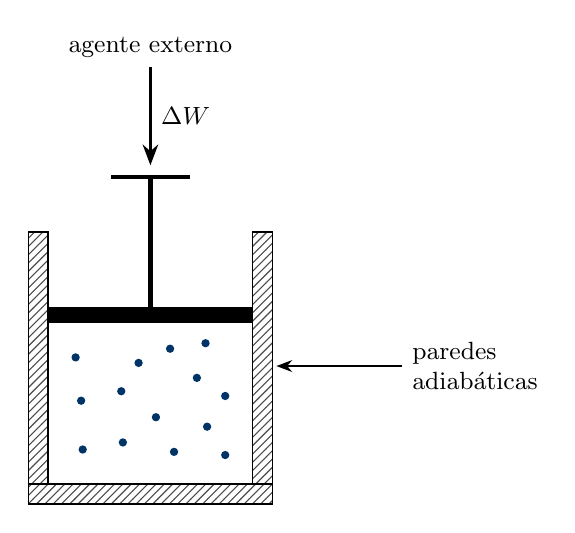
\begin{tikzpicture}
  \path[adia] (-0.25,-0.25) rectangle (2.85,0);
  \path[adia] (-0.25,0) rectangle (0,3.2);
  \path[adia] (2.6,0) rectangle (2.85,3.2);
  \fill[black] (0,2.05) rectangle (2.6,2.25);
  \draw[line width=1.6pt] (1.3,2.25) -- (1.3,3.9);
  \draw[line width=1.6pt] (0.8,3.9) -- (1.8,3.9);
  \fill[UGblue] (0.95,0.53) circle (1.5pt);
  \fill[UGblue] (1.60,0.41) circle (1.5pt);
  \fill[UGblue] (1.37,0.85) circle (1.5pt);
  \fill[UGblue] (0.42,1.06) circle (1.5pt);
  \fill[UGblue] (0.44,0.44) circle (1.5pt);
  \fill[UGblue] (1.15,1.54) circle (1.5pt);
  \fill[UGblue] (1.55,1.72) circle (1.5pt);
  \fill[UGblue] (2.25,0.37) circle (1.5pt);
  \fill[UGblue] (2.02,0.73) circle (1.5pt);
  \fill[UGblue] (0.93,1.18) circle (1.5pt);
  \fill[UGblue] (1.89,1.35) circle (1.5pt);
  \fill[UGblue] (0.35,1.61) circle (1.5pt);
  \fill[UGblue] (2.00,1.79) circle (1.5pt);
  \fill[UGblue] (2.25,1.12) circle (1.5pt);
  \draw[->,line width=1pt] (1.3,5.3) -- (1.3,4.05) node[midway,right] {$\Delta W$};
  \node[above] at (1.3,5.3) {agente externo};
  \draw[->,line width=0.6pt] (4.5,1.5) node[right,align=left] {paredes\\adiabáticas} -- (2.9,1.5);
\end{tikzpicture}
\end{document}
